%%% LaTeX Template: Article/Thesis/etc. with colored headings and special fonts
%%%
%%% Source: http://www.howtotex.com/
%%% Feel free to distribute this template, but please keep to referal to http://www.howtotex.com/ here.
%%% February 2011
%%%
%%% Modified January 2016 by CDM

%%%  Preamble
\documentclass[11pt,letterpaper]{article}
\usepackage[margin=1.0in]{geometry}
\usepackage[T1]{fontenc}
\usepackage[bitstream-charter]{mathdesign}
\usepackage[latin1]{inputenc}					
\usepackage{amsmath}						
\usepackage{xcolor}
\usepackage{cite}
\usepackage{hyphenat}
\usepackage{graphicx}
\usepackage{float}
\usepackage{subfigure}
\usepackage{sectsty}
\usepackage[compact]{titlesec} 
\usepackage[tablegrid]{vhistory}
\usepackage{pbox}
\allsectionsfont{\color{accentcolor}\scshape\selectfont}

%%% Definitions
\definecolor{accentcolor}{rgb}{0.0,0.0,0.5} 
\newcommand{\teamname}{Resonance}
\newcommand{\productname}{LTunes}
\newcommand{\coursename}{CSE 4317: Senior Design II}
\newcommand{\semester}{Spring 2020}
\newcommand{\docname}{Architectural Design Specification}
\newcommand{\department}{Department of Computer Science \& Engineering}
\newcommand{\university}{The University of Texas at Arlington}
\newcommand{\authors}{Amir Dhungana \\ Anish Yonjan \\ Roberto Torres \\ Raul Jimenez \\ Rabinson Shrestha \\ Nikhil Purohit}

%%% Headers and footers
\usepackage{fancyhdr}
	\pagestyle{fancy}						% Enabling the custom headers/footers
\usepackage{lastpage}	
	% Header (empty)
	\lhead{}
	\chead{}
	\rhead{}
	% Footer
	\lfoot{\footnotesize \teamname \ - \semester}
	\cfoot{}
	\rfoot{\footnotesize page \thepage\ of \pageref{LastPage}}	% "Page 1 of 2"
	\renewcommand{\headrulewidth}{0.0pt}
	\renewcommand{\footrulewidth}{0.4pt}

%%% Change the abstract environment
\usepackage[runin]{abstract}			% run in option for a run-in title
%\setlength\absleftindent{30pt}			% left margin
%\setlength\absrightindent{30pt}		% right margin
\abslabeldelim{\quad}	
\setlength{\abstitleskip}{-10pt}
\renewcommand{\abstractname}{}
\renewcommand{\abstracttextfont}{\color{accentcolor} \small \slshape}	% slanted text

%%% Start of the document
\begin{document}

%%% Cover sheet
{\centering \huge \color{accentcolor} \sc \textbf{\department \\ \university} \par}
\vspace{1 in}
{\centering \huge \color{accentcolor} \sc \textbf{\docname \\ \coursename \\ \semester} \par}
\vspace{0.5 in}
\begin{figure}[h!]
	\centering
   	
\includegraphics[width=0.60\textwidth]{images/logo}
\end{figure}
\vspace{0.5 in}
{\centering \huge \color{accentcolor} \sc \textbf{\teamname \\ \productname} \par}
\vspace{0.5 in}
{\centering \large \sc \textbf{\authors} \par}
\newpage


%\vspace{1 in}
%\centerline{January 13th, 2012}
%\newpage

%%% Revision History
\begin{versionhistory}
  	\vhEntry{0.1}{11.02.2019}{AD}{document creation}
  	\vhEntry{0.2}{11.06.2019}{AY|AD}{complete draft}
  	\vhEntry{1.0}{11.08.2019}{AY|AD}{official release}
  	\vhEntry{1.1}{05.10.2020}{AY}{added design review requests}
\end{versionhistory}
\newpage

%%% Table of contents
\setcounter{tocdepth}{2}
\tableofcontents
\newpage

%%% List of figures and tables (optional)
\listoffigures
\listoftables
\newpage

%%% Document sections
\section{Introduction}
Your introduction should describe your product concept in sufficient detail that the architectural design will be easy to follow. The introduction may include information used in the first sections of your SRS for this purpose. At a minimum, ensure that the product concept, scope and key requirements are described.
\newpage
\section{System Overview}
This section should reintroduce the full data flow diagram from the architectural specification, and discuss at a high level the purpose of each layer. You do not need to include a subsection for each layer, a 1 - 2 paragraph recap is sufficient.

\begin{figure}[h!]
	\centering
 	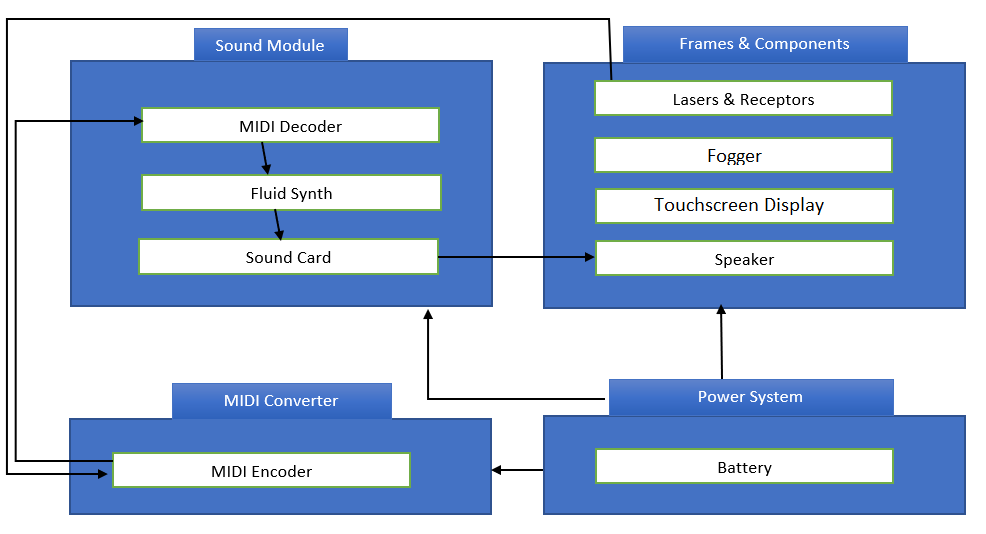
\includegraphics[width=0.90\textwidth]{images/data_flow}
 \caption{System architecture}
\end{figure}

\newpage
\section{Subsystem Definitions \& Data Flow}
This section breaks down your layer abstraction to another level of detail. Here you grapically represent the logical subsytems that compose each layer and show the interactions/interfaces between those subsystems. A subsystem can be thought of as a programming unit that implements one of the major functions of the layer. It, therefore, has data elements that serve as source/sinks for other subsystems. The logical data elements that flow between subsystems need to be explicitly defined at this point, beginning with a data flow-like diagram based on the block diagram.

\begin{figure}[h!]
	\centering
 	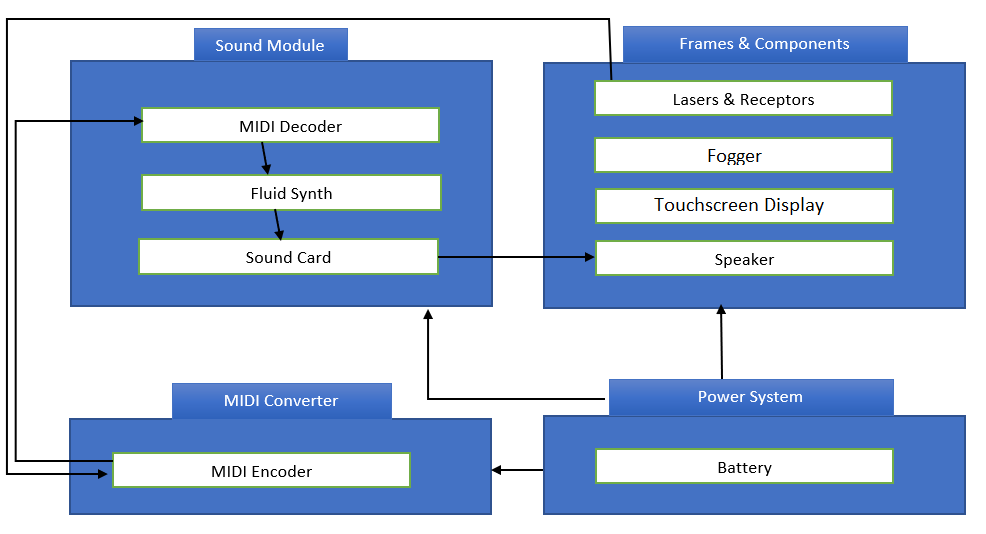
\includegraphics[width=\textwidth]{images/data_flow}
 \caption{A simple data flow diagram}
\end{figure}

\newpage
\section{Power System Layer Subsystems}
The details about the subsystem included in the power layer are discussed below. We are opting to go with centralizing the raspberry pi as the main power source. It will sort of act as a power source to all the other components and it itself is powered by plugging to an external outlet.  

\subsection{Raspberry Pi}
Raspberry Pi is the only subsystem component included in this layer. It will act as the power source for all the components. It will be connected to other components via wires and cables.

\subsubsection{Assumptions}
The Raspberry Pi will be able to provide enough power to run all the components of the instrument for a reasonable amount time without difficulties. It will have access to external outlet to power itself.

\subsubsection{Responsibilities}
It is responsible for providing adequate power to all the components of the device.

\subsubsection{Subsystem Interfaces}
Input and output for the Raspberry Pi subsystem are mentioned below.

\begin {table}[H]
\caption {Subsystem interfaces} 
\begin{center}
    \begin{tabular}{ | p{1cm} | p{6cm} | p{3cm} | p{3cm} |}
    \hline
    ID & Description & Inputs & Outputs \\ \hline
    \#xx & Raspberry Pi  & \pbox{3cm}{120V outlet} & \pbox{3cm}{2A DC Power}  \\ \hline
    \end{tabular}
\end{center}
\end{table}

\newpage
\section{Frame and Component Layer Subsystems}
Frames and components make up the external outlook of the device. Furthermore, it is the layer that allows the user to interact with the device. It consists of three subsystems which include laser and receptors, mister and speakers. 

\subsection{Laser and receptors}
This subsystem comprises of laser beams and receptors to detect the interference for the same. It consists of laser diodes pointed towards the photo resistors.  The receptors will not only detect the breaking of the beam, but also the number or note of the beam interfered. This information is then transferred to MIDI encoder for further analysis.

\begin{figure}[h!]
	\centering
 	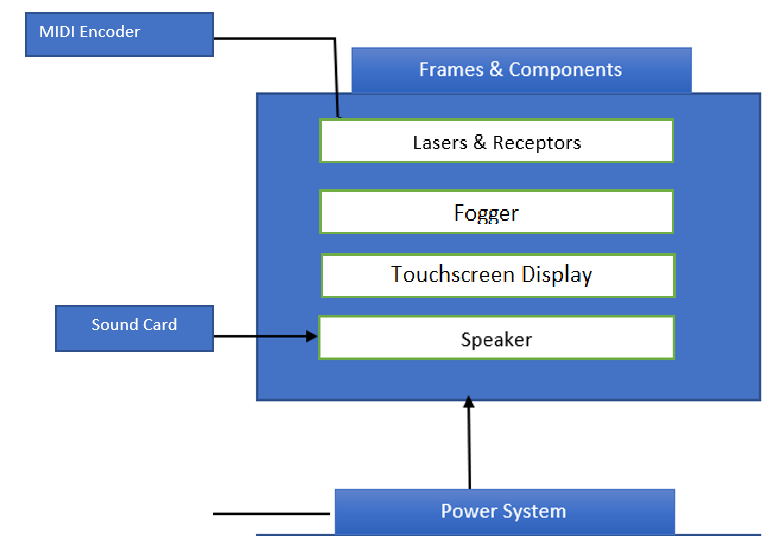
\includegraphics[width=0.60\textwidth]{images/Frame}
 \caption{Laser and Receptors subsystem description diagram}
\end{figure}

\subsubsection{Assumptions}
It is assumed that laser diodes are properly placed in position with respect to resistors. All the laser diodes are functioning properly, and no external factors are causing the interference other than the user.

\subsubsection{Responsibilities}
It is responsible for production of laser beams as well as recording of the breakage of laser beams. Furthermore, it should transmit those records to MIDI encoder.

\subsubsection{Subsystem Interfaces}
An external power supply is connected to the subsystem using breadboard or hookup wires. 

A USB to MIDI cable is used to connect the subsystem to encoder.

\begin {table}[H]
\caption {Subsystem interfaces} 
\begin{center}
    \begin{tabular}{ | p{1cm} | p{6cm} | p{3cm} | p{3cm} |}
    \hline
    ID & Description & Inputs & Outputs \\ \hline
    \#01 & Laser Diodes & \pbox{3cm}{Power supply} & \pbox{3cm}{Laser beams }  \\ \hline
    \#02 & Receptors & \pbox{3cm}{Interference} & \pbox{3cm}{Signals}  \\ \hline
    \#03 & MIDI Interface & \pbox{3cm}{Signals} & \pbox{3cm}{Event Messages }  \\ \hline
    \end{tabular}
\end{center}
\end{table}

\subsection{Fogger}
It consists of a mini vape model that will be produce fog or vape which enhances the visibility of the lasers. It will take power source from Raspberry Pi. It will use the power to convert vape juice inside of it to fog.

\begin{figure}[h!]
	\centering
 	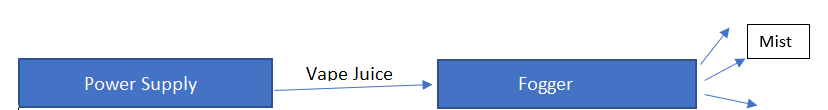
\includegraphics[width=0.60\textwidth]{images/fogger}
 \caption{Laser and Receptors subsystem description diagram}
\end{figure}

\subsubsection{Assumptions}
It is assumed that there is enough vape juice inside the fogger and adequate power supply.

\subsubsection{Responsibilities}
It is responsible for emitting fog or mist which will be used to make the lasers visible to naked eye in well-lit room.

\subsubsection{Subsystem Interfaces}
Power is given to the mister through Raspberry Pi.

Fogger takes input from the vape juice which is converted into mist. 


\begin {table}[H]
\caption {Subsystem interfaces} 
\begin{center}
    \begin{tabular}{ | p{1cm} | p{6cm} | p{3cm} | p{3cm} |}
    \hline
    ID & Description & Inputs & Outputs \\ \hline
    \#01 & Fogger & \pbox{3cm}{Vape juice} & \pbox{3cm}{Mist}  \\ \hline 
   \end{tabular}
\end{center}
\end{table}

\subsection{Speaker system}
It consists of single or multiple speakers which will be hooked up to the sound module. It will give the audio output for any presets or interference created by the user.

\begin{figure}[h!]
	\centering
 	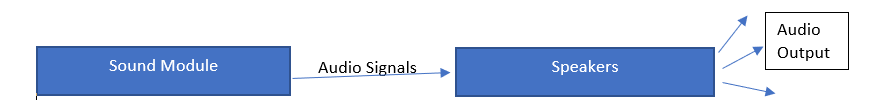
\includegraphics[width=0.60\textwidth]{images/Speaker}
 \caption{Laser and Receptors subsystem description diagram}
\end{figure}

\subsubsection{Assumptions}
Speakers are fairly new and the device is played in quiet place so as to ensure that there is no background noise.

\subsubsection{Responsibilities}
It is responsible for producing clear audio output.

\subsubsection{Subsystem Interfaces}
It receives the signals from the sound module and produces the resulting audio output based on the signals fed to it. 


\begin {table}[H]
\caption {Subsystem interfaces} 
\begin{center}
    \begin{tabular}{ | p{1cm} | p{6cm} | p{3cm} | p{3cm} |}
    \hline
    ID & Description & Inputs & Outputs \\ \hline
    \#01 & Speakers & \pbox{3cm}{Audio Signals} & \pbox{3cm}{Audio Output}  \\ \hline 
   \end{tabular}
\end{center}
\end{table}

\subsection{Touchscreen Display}
It consists of a 6" inch touchscreen monitor that is used for toggling between presets and changing the settings. It is also useful for viewing the current settings and preset. The UI is based on Kiwi UI for the display.

\begin{figure}[h!]
	\centering
 	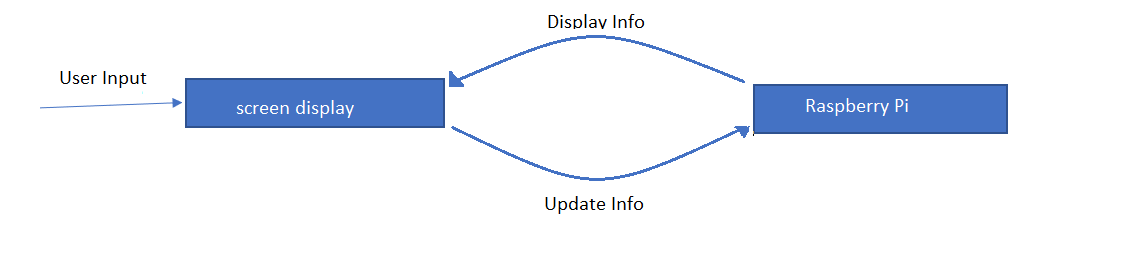
\includegraphics[width=0.60\textwidth]{images/screen}
 \caption{Laser and Receptors subsystem description diagram}
\end{figure}

\subsubsection{Assumptions}
It is powered by the Raspberry Pi and it can take inputs from the screen display. 

\subsubsection{Responsibilities}
It is responsible for toggling between presets and changing the settings.

\subsubsection{Subsystem Interfaces}
It is connected directly to the Raspberry Pi via a USB-C cable.

It displays the information on the screen and also takes input from user through the same screen 


\begin {table}[H]
\caption {Subsystem interfaces} 
\begin{center}
    \begin{tabular}{ | p{1cm} | p{6cm} | p{3cm} | p{3cm} |}
    \hline
    ID & Description & Inputs & Outputs \\ \hline
    \#01 & Touchscreen Display & \pbox{3cm}{Raspberry Pi} & \pbox{3cm}{display info}  \\ \hline 
    \#01 & Touchscreen Display & \pbox{3cm}{user input} & \pbox{3cm}{update info}  \\ \hline 
   \end{tabular}
\end{center}
\end{table}


\newpage
\section{MIDI Layer Subsystems}
In this section, the layer is described in some detail in terms of its specific subsystems. Describe each of the layers and its subsystems in a separate chapter/major subsection of this document. The content of each subsystem description should be similar. Include in this section any special considerations and/or trade-offs considered for the approach you have chosen.

\subsection{MIDI encoder}
The MIDI encoder gets the signal from the laser receptors, converts it to MIDI data and sends to the Raspberry Pi for the output. This converts the laser receptor signals to MIDI data in order to convert it to sound data.  

\begin{figure}[h!]
	\centering
 	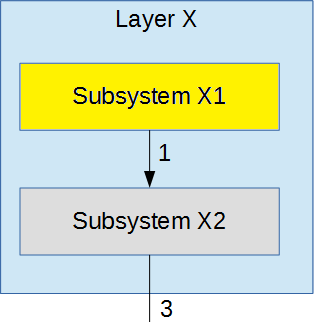
\includegraphics[width=0.60\textwidth]{images/subsystem}
 \caption{MIDI encoder subsystem description diagram}
\end{figure}

\subsubsection{Assumptions}
The MIDI encoder is connected to the Pi and the laser receptors via usb-A cable. It also has a built-in software that converts the data automatically.

\subsubsection{Responsibilities}
The laser recptors, when it detects an interference, sends signal to the MIDI encoder. Here, the encoder converts the signal data it received to a MIDI data so it can be maniplated to different sounds with the sound modules.

\subsubsection{Subsystem Interfaces}
Each of the inputs and outputs for the subsystem are defined here. Create a table with an entry for each labelled interface that connects to this subsystem. For each entry, describe any incoming and outgoing data elements will pass through this interface.

\begin {table}[H]
\caption {Subsystem interfaces} 
\begin{center}
    \begin{tabular}{ | p{1cm} | p{6cm} | p{3cm} | p{3cm} |}
    \hline
    ID & Description & Inputs & Outputs \\ \hline
    \#xx & Description of the interface/bus & \pbox{3cm}{input 1 \\ input 2} & \pbox{3cm}{output 1}  \\ \hline
    \#xx & Description of the interface/bus & \pbox{3cm}{N/A} & \pbox{3cm}{output 1}  \\ \hline
    \end{tabular}
\end{center}
\end{table}



\newpage
\section{Sound Modules Layer Subsystems}
In this section, the layer is described in some detail in terms of its specific subsystems. Describe each of the layers and its subsystems in a separate chapter/major subsection of this document. The content of each subsystem description should be similar. Include in this section any special considerations and/or trade-offs considered for the approach you have chosen.

\subsection{MIDI decoder}
pending
\begin{figure}[h!]
	\centering
 	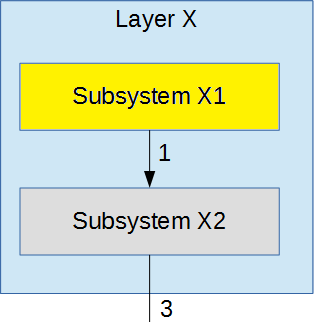
\includegraphics[width=0.60\textwidth]{images/subsystem}
 \caption{Example subsystem description diagram}
\end{figure}

\subsubsection{Assumptions}
pending

\subsubsection{Responsibilities}
pending

\subsubsection{Subsystem Interfaces}
pending

\begin {table}[H]
\caption {Subsystem interfaces} 
\begin{center}
    \begin{tabular}{ | p{1cm} | p{6cm} | p{3cm} | p{3cm} |}
    \hline
    ID & Description & Inputs & Outputs \\ \hline
    \#xx & Description of the interface/bus & \pbox{3cm}{input 1 \\ input 2} & \pbox{3cm}{output 1}  \\ \hline
    \#xx & Description of the interface/bus & \pbox{3cm}{N/A} & \pbox{3cm}{output 1}  \\ \hline
    \end{tabular}
\end{center}
\end{table}

\subsection{Speaker}
The speaker gives the final output of the laser harp. After all the processing of the data in the raspberry pi, the pi sends the final output of the sound signal to the speakers. The speakers produce the desired sound as output. 

\begin{figure}[h!]
	\centering
 	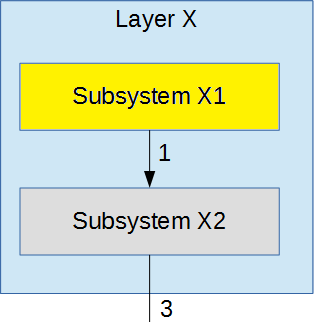
\includegraphics[width=0.60\textwidth]{images/subsystem}
 \caption{Example subsystem description diagram}
\end{figure}

\subsubsection{Assumptions}
The speaker is connected via USB A cable to the pi. It is also powered by the same battery powering the Raspberry Pi.

\subsubsection{Responsibilities}
The speaker should produce decent sound output with no interference. It should be loud enough so the sound can be heard in a conference hall. 

\subsubsection{Subsystem Interfaces}
The speaker gets analog signals from the raspberry pi and converts it into sound waves as output. This is the final output of the system. The speaker is connected via USB A cable to the system.

\begin {table}[H]
\caption {Subsystem interfaces} 
\begin{center}
    \begin{tabular}{ | p{1cm} | p{6cm} | p{3cm} | p{3cm} |}
    \hline
    ID & Description & Inputs & Outputs \\ \hline
    \#xx & Description of the interface/bus & \pbox{3cm}{input 1 \\ input 2} & \pbox{3cm}{output 1}  \\ \hline
    \#xx & Description of the interface/bus & \pbox{3cm}{N/A} & \pbox{3cm}{output 1}  \\ \hline
    \end{tabular}
\end{center}
\end{table}

\subsection{FluidSynth}
FluidSynth is a real-time software synthesizer based on the SoundFont 2 specifications and has reached widespread distribution. It converts the MIDI signals to produce desired sound waves.

\begin{figure}[h!]
	\centering
 	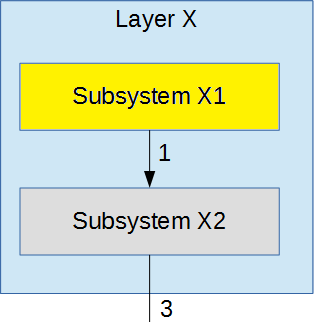
\includegraphics[width=0.60\textwidth]{images/subsystem}
 \caption{Example subsystem description diagram}
\end{figure}

\subsubsection{Assumptions}
The software already has default preset sounds built-in. It also has the functionality manipulate the sound to produce various sound effects. Also it is free, open source and easy to use.

\subsubsection{Responsibilities}
The software is used to convert MIDI signals to sound waves. It should have multiple different sound effects and create a wide range of sound octaves in different formats.

\subsubsection{Subsystem Interfaces}
The software is downloaded and installed into the raspberry pi. It is supported by the Raspian OS.

\begin {table}[H]
\caption {Subsystem interfaces} 
\begin{center}
    \begin{tabular}{ | p{1cm} | p{6cm} | p{3cm} | p{3cm} |}
    \hline
    ID & Description & Inputs & Outputs \\ \hline
    \#xx & Description of the interface/bus & \pbox{3cm}{input 1 \\ input 2} & \pbox{3cm}{output 1}  \\ \hline
    \#xx & Description of the interface/bus & \pbox{3cm}{N/A} & \pbox{3cm}{output 1}  \\ \hline
    \end{tabular}
\end{center}
\end{table}

\newpage

\end{document}
